\documentclass[eng]{class}

% Publication Title
\title{EDI: First/Second Lab Report}
% Short title for the header (copy the main title if it is not too long)
\shorttitle{EDI: First/Second Lab Report}
       
% Authors
\author[1]{D. Ligari 518592}
% Author Affiliations
\affil[1]{University of Pavia, Department of Computer Engineering (Data Science), Pavia, Italy}
% Surname of the first author of the manuscript
\firstauthor{Ligari}
%Contact Author Information
\contactauthor{D. Ligari} % Name and surname of the contact author
\email{davide.ligari01@universitadipavia.it} % Contact Author Email
% Publication data (will be defined in the edition)
\publicationdate{\today}
% Place your particular definitions here
\newcommand{\vect}[1]{\mathbf{#1}}  % vectors


\abstract{  This report presents two analyses of network performance with regards to ProtonVPN servers and DNS servers.
The first analysis evaluates the performance of various ProtonVPN servers and investigates the impact of server location on network performance.
To accomplish this, measurements of latency, packet loss, and network bandwidth were taken using tools such as Speedtest-cli, Ping, and MTR.
The second analysis focuses on DNS performance, beginning with an overview of DNS functionality
and studying the contents of DNS queries and responses, followed by an evaluation of the performance of different DNS servers and protocols.\\
During the investigation, the latency, packet loss, and DNS query resolution time of different DNS servers was measured.
The results provide insights into optimal server selection to maximize performance, privacy and security of the user.}
\keywords{
  VPN • Performance • Speedtest • Ping • MTR • DNS • dig • dnseval • DNSSEC • DoT • DoH}
\date{\today}
% Start document
\begin{document}
\pagenumbering{arabic}
% Include title, authors, abstract, etc.
\maketitle
\tableofcontents
\thispagestyle{FirstPage}
%Figures and tables must be cited in the text and explained in detail. Do not forget to add a caption to each figure/table/
\vspace{\baselineskip}
\section{Performance of Proton VPN}
\firstword{V}{irtual} Private Networks (VPN) have become increasingly popular in recent years due to the growing concern over online privacy and security.
They allow users to create a secure and private connection to the internet, thereby protecting their sensitive data from prying eyes.
Additionally, this technology can help bypass geographic restrictions and censorship, allowing users to access content that may be restricted in their location.
VPN works by routing a user's internet traffic through an encrypted tunnel to a server located in another place,
which then forwards the user's traffic to its intended destination.
However, while virtual private network can provide increased security and privacy, it may also introduce overhead
that can lead to high latency and poor network performance, particularly if the server location is not carefully chosen.
In this report, the performance of different VPN servers, provided by ProtonVPN, are compared to a local internet connection.
By comparing the performance of these connections, this report aims to provide valuable insights into the effectiveness of VPNs and assist users in selecting the best server location for their needs.
\subsection{Tools used}
\textbf{Ping} \\
Ping is a network utility tool used to test the connectivity between two networked devices.
It sends a small packet of data to a specific IP address or hostname and measures the time it takes for that packet to be received and returned.
The result shows the round trip time (RTT), as well as the number of packets sent and received, and any packet loss that may have occurred.\\
While it is a useful tool for testing network connectivity, it has some limitations,
it uses the ICMP protocol to send and receive packets, which may not always be allowed by network firewalls or routers, and it does not support different protocols like TCP or UDP.
This means that if a network is configured to block ICMP traffic, the ping command may not work.
Moreover ping provides only basic information about network connectivity, it does not provide information about bandwidth or the structure of the network.\\
\\
\pagestyle{OtherPage}

\noindent
\textbf{Traceroute} \\
The "traceroute" is another tool used to trace the path that packets take from one networked device to another.
It sends a series of packets with increasing Time-to-Live (TTL) values and records the IP addresses of the devices that process the packets along the way.
By analyzing the sequence of IP addresses returned by the traceroute command,
it is possible to determine the path that packets take through the network and identify any network devices that may be causing delays or packet loss.
The traceroute command is useful for troubleshooting network issues, identifying network bottlenecks, and determining the route that packets take through the network.
However, it may be inaccurate, because, due to network congestion or routing changes,
the path taken by packets may not always be the same as the path taken by traceroute packets.
In addition, traceroute provides only basic information about the path of packets through the network,
it only shows the path between the vantage point and the target point, not the complete structure of the network.
For this reason it is crucial the choice of the vantage and target points.\\
\\
\textbf{MTR} \\
The mtr (short for "My traceroute") is a tool that combines the functionality of the "ping" and "traceroute" commands.
It continuously sends packets to a destination IP address or hostname and displays  in real-time
different statistics, such as average and standard deviation of the latency for each hop, percentage of packet loss.
Mtr works by sending a series of ICMP packets with increasing TTL values, similar to the traceroute command.
However, unlike traceroute, mtr does not stop after reaching the destination device; instead,
it continues to send packets and displays the round-trip time and packet loss for each hop along the route.
Mtr also includes additional features such as the ability to save the results to a file for later analysis.
Despite this, mtr has the same limitations as traceroute.\\
\\
\textbf{Speedtest} \\
The speedtest-cli is a command-line interface tool used to test the speed of an internet connection.
It uses a server-client model to measure the download and upload speeds, as well as the latency of an internet connection.
Speedtest-cli works by connecting to a nearby server and downloading and uploading a series of files.
It then calculates the download and upload speeds based on the time taken to transfer the files and the size of the files.
It also measures the latency of the connection by sending and receiving small data packets.
Speedtest-cli provides detailed information about the internet connection, including the download speed, upload speed, and ping time.
\subsection{Methodology and experimental setup}
The purpose of this experiment was to evaluate the performance of three ProtonVPN servers, located in US, Netherlands and Japan,
and examine how the choice of server location impacts network performance when accessing Google.com. The experiment was conducted on the researcher's laptop, located in Pavia.\\
To achieve this goal, several metrics were measured, including the latency of the network with and without using the VPNs,
differences in the paths taken to reach the target point, the bandwidth of the user's network and the VPN servers.\\
To measure network latency, the ping command was used.
The mtr tool was utilized to observe the path taken to reach the target point and identify any differences in the paths when using different VPN servers.
The speedtest command was used to measure the bandwidth of both the user's network and the VPN servers.
\subsection{Overall latency analysis}
Latency refers to the amount of time it takes for a data packet to travel from its source to its destination across a network.
It is the delay between the initiation of a network request and the response received.
High latency can lead to slow response times, poor network performance, and user frustration.
\\Latency data were obtained by using the ping command (shown below), which sends 200 packets, one per second, to a Google server and store the results into a file.
To make the data independent of external factors, such as network congestion, the ping command was executed at three different times of the day for each VPN servers.
\begin{lstlisting}
  ping -c 200 google.com >> ./ping/ping_JP.txt
\end{lstlisting}
\noindent
It results that network latency is strongly influenced by the distance between the client and the server, shown in Figure \ref*{fig-1}.
In particular, network latency is higher when the client is in Italy and the server in Japan or the United States,
This is the expected behavior, because if two endpoints are located in the same country or Continent, like Italy and Netherlands, the data only needs to travel through a few devices and links, resulting in a short latency.
However, if the endpoints are located on opposite sides of the world, like Italy and Japan or US, the data needs to travel across multiple continents and through many devices and links,
resulting in a much longer latency.
\begin{figure}[H]
  \centering
  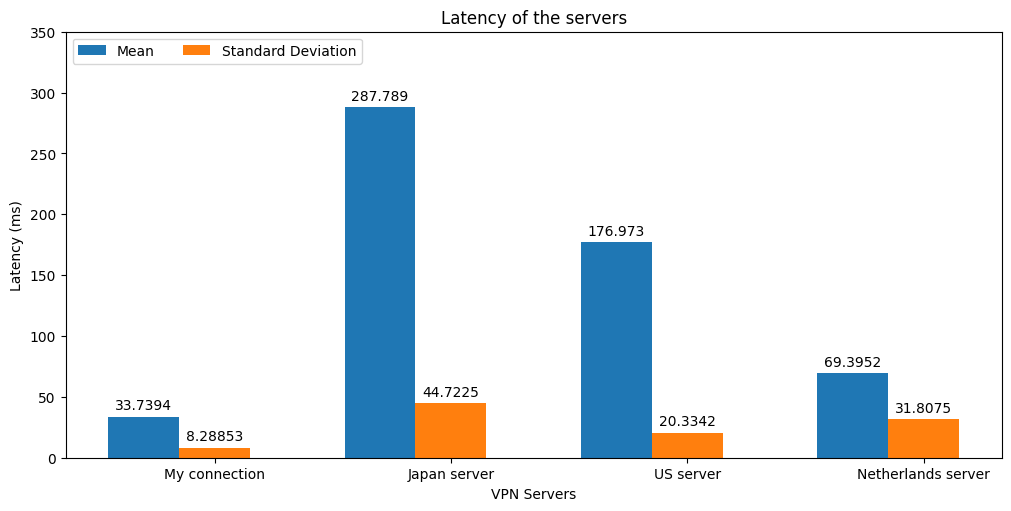
\includegraphics[width=.7\columnwidth]{images/ServerLatency.png}
  \caption{Mean and standard deviation of the latency of the researcher's network and the VPN servers}
  \label{fig-1}
\end{figure}
\subsection{Latency analysis for each hop}
While analyzing the overall latency of a network using tools such as ping can provide valuable insights into network performance,
it is also important to consider the latency for each hop in the network.
A hop refers to each point in the network where data passes through a device such as a router or switch. By measuring the latency at each hop,
network administrators can pinpoint where performance issues are occurring and take steps to address them.
For this reason, the mtr tool was used to measure the latency of each hop in the networks.
The mtr command was executed in different hours of a day, for each VPN server, sending 300 packets to Google.com and storing the results into a file.
\begin{lstlisting}
  mtr --json  -c 300  google.com >> mtr_NL.json
\end{lstlisting}
The graphs in Figures \ref{fig-2} to \ref{fig-3} clearly demonstrate that the US server and the researcher's network are more reliable than the other servers,
as they exhibit lower average latency and smaller standard deviation. However, a closer inspection of hops 2 and 3 in the researcher's network is necessary,
as they demonstrate a high standard deviation.
It is important to note that the path taken by traceroute packets may change, and hops may not always be the same,which can affect the standard deviation.
In contrast, the NL server, while having a lower average latency, suffers from a high standard deviation, indicating unstable performance.
On the other hand, the JP server has a very high average latency coupled with a low standard deviation, which suggests that its performance is poor and consistent.
Overall, the graphs provide valuable information about network performance, highlighting the importance of both average latency and standard deviation.
Further analysis is needed to determine the root causes of any performance issues.
\begin{figure}[H]
  \centering
  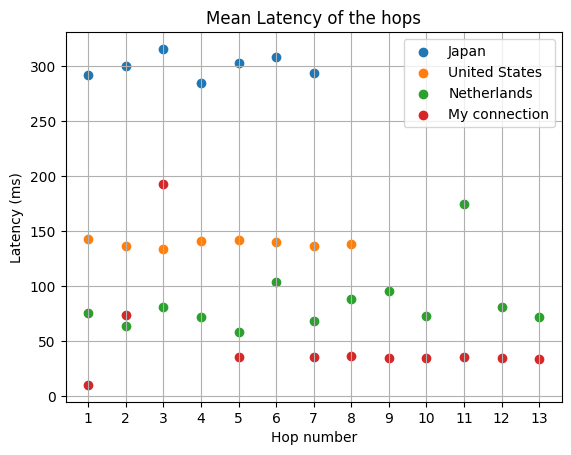
\includegraphics[width=.7\columnwidth]{images/meanLHops.png}
  \caption{Mean of the hop latency of each network}
  \label{fig-2}
\end{figure}
\begin{figure}[H]
  \centering
  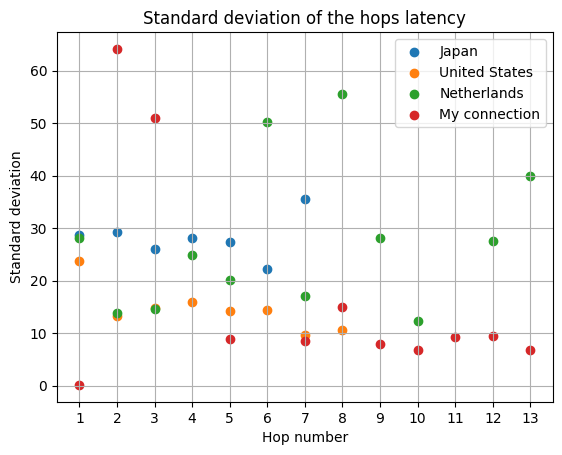
\includegraphics[width=.7\columnwidth]{images/varLHops.png}
  \caption{standard deviation of the hop latency of each network}
  \label{fig-3}
\end{figure}

\subsection{Bandwidth analysis}
Bandwidth refers to the maximum amount of data that can be transmitted over a network connection in a given amount of time.
It is typically measured in bits per second (bps) or bytes per second (Bps).
Bandwidth data were obtained by using the speedtest command (shown below),which returns the data and stores them in a JSON file.
In order to have consistent data, this command was executed many times during the day and for each VPN servers.
\begin{lstlisting}
  speedtest-cli --json  --server 6554 >> speedtest.json
\end{lstlisting}
Figure \ref*{fig-4} displays the bandwidth measurements for each network.
The Netherlands has the highest bandwidth, followed by the US, the researcher's connection, and Japan.\\
While network characteristics such as network congestion, network type (wired or wireless),
and network hardware are the primary factors that affect available bandwidth, distance can also play a role in determining the quality of the connection.
As distance increases, the time it takes for data to travel between the client and server increases as well,
which can result in higher latency and potentially lower available bandwidth due to increased signal degradation, interference, and other factors.
However, the impact of distance can be trascured, because the speedtest servers has been selected in order to keep the distance constant for each VPN server.\\
When considering the impact of distance on bandwidth, it is important to note that the distance referred to here is the distance between the VPN server and
the server selected by the speed test to perform the analysis.

\begin{figure}[H]
  \centering
  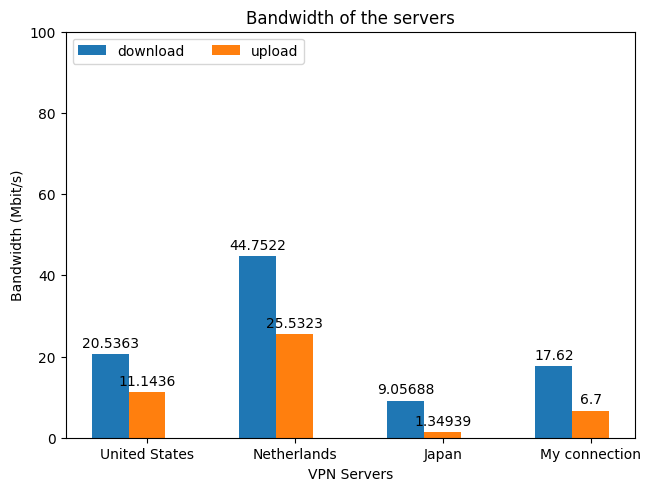
\includegraphics[width=.7\columnwidth]{images/ServerBandwidth.png}
  \caption{Mean of download and upload speed of the researcher's network and the VPN servers}
  \label{fig-4}
\end{figure}
\section{Evaluation of DNS Functionalities}
The Domain Name System (DNS) is an essential component of the Internet infrastructure that translates domain names into IP addresses,
enabling users to access websites by simply typing in the domain name instead of the IP address.
Understanding DNS and its functionality is crucial to understand how the Internet works and its underlying structure.
DNS is a hierarchical, distributed database system that manages the mapping of domain names to IP addresses.
It consists of several components, including DNS servers, resolvers, and recursive resolvers, each performing a specific function in the translation process.
With its critical role in Internet connectivity, DNS performance and reliability are essential for ensuring optimal user experience and maintaining network security.

\subsection{Tools used}
\textbf{Dig} \\
The dig command (short for "domain information groper") is a popular network administration tool used to perform DNS queries.
It allows users to perform DNS lookups to check DNS records and obtain information about DNS configurations.
It is a versatile tool that allows users to specify different query types, such as A, AAAA, MX, TXT, and others.
It can also be used to perform reverse DNS queries, where an IP address is used to retrieve the corresponding domain name.
In addition to provide detailed DNS query results, the dig command can also be used to troubleshoot DNS issues, such as misconfigured DNS servers,
slow DNS resolution times, or DNS cache issues.\\
\\
\textbf{Dnstraceroute} \\
Dnstraceroute is a command-line tool used to trace the path that DNS queries take when traversing the Internet.
It works similarly to the traditional traceroute command, but instead of tracing the path that packets take,
it traces the path that DNS queries take from the local machine to the destination server.
Dnstraceroute sends DNS queries with increasing TTL (Time to Live) values,
which causes each hop along the path to respond with an ICMP message indicating the hop's IP address.
Its limitations are the same as traceroute,it may be inaccurate, because, due to network congestion or routing changes.\\
\\
\textbf{Dnseval} \\
Dnseval is a powerful and versatile tool that enables users to perform a predefined number of DNS queries to a specified domain name,
providing valuable insights into the performance and reliability of DNS servers.
With Dnseval, users can measure the time it takes to resolve a domain name, and obtain detailed statistics such as the average, minimum,
and maximum query response times, as well as the percentage of failed queries.
It also allows  to select the protocol to use (UDP, TCP, DOT or DOH), the type of query to perform (A, AAAA, MX, TXT, etc.),
and choose whether to enable DNSSEC.\\
\\
\textbf{Whois} \\
The whois command allows users to look up information about domain names, IP addresses, and other network-related entities.
The command retrieves publicly available data from a WHOIS database, which contains information such as the registered owner of the domain name,
the domain registrar, the date of creation and expiration of the domain name, and the contact information for the domain owner.
Whois is commonly used by network administrators, domain owners, and law enforcement agencies to gather information
about network entities and to troubleshoot issues related to domain registration, ownership, and use.\\

\subsection{Methodology and experimental setup}
In the first part of this experiment, various active tests were conducted to analyze the contents of DNS queries and responses,
and to examine the variations that occur when using different local name servers.
In the second part of the experiment, performance tests were conducted to investigate the impact of different factors on overall DNS latency,
such as the choice of transport protocol, the location of the name server, and the use of encrypted transmission.
By examining these different aspects of DNS performance, a better understanding of optimal server selection and network configurations can be obtained.

\subsection{Active experiments}
During  this experiment, there were used different public name servers.
The most important are shown in the following table.

\rowcolors{2}{green!8}{green!18}
\begin{table}[H]
  \centering
  \begin{tabular}{|c|c|}
    \hline
    \linewidth=0cm
    Name server       & ip              \\
    \hline
    Google            & 8.8.4.4         \\
    Quad9             & 149.112.112.112 \\
    OpenDNS           & 208.67.220.220  \\
    Comodo Secure DNS & 8.20.247.20     \\
    \hline
  \end{tabular}
  \caption{Local name servers used}\label{tab-1}
\end{table}
\subsubsection*{1. Query the DNS to obtain the IP addresses of achille.unipv.it and of another hostname in the TLD domain it, are the answers authoritative? Why?}
The dig command (shown below) was utilized to obtain information about a domain name by passing arguments that include the local name server
to be used and the domain name for which we want to retrieve information.
In this experiment, several local name servers, including the ones listed above, were used, as well as the one from the University of Pavia.
Two domain names, achille.unipv.it and www.istat.it, were used for this purpose.
\begin{lstlisting}
  dig  @8.8.4.4 achille.unipv.it
\end{lstlisting}
The DNS answers are composed of various fields that provide information about the domain name, such as the IP address associated with it,
the type of query, and the time-to-live (TTL). \\
To determine if an answer is authoritative, we need to examine the flags and check if the AA (Authoritative Answer) flag is present (Table \ref*{tab-2}).
Analyzing the domain name achille.unipv.it, we find that only the local name server of the University of Pavia provides an authoritative answer.
This is because the university's server is responsible for managing the domain unipv.it, which includes the subdomain achille.unipv.it.
In contrast, for the domain name www.istat.it, none of the local name servers used provide an authoritative answer because they do not have authority over that domain.\\
Interestingly, when the university's server is queried for information on istat.it, it does not return the requested information.
This is because the university's server does not support recursion, which  is a mechanism that allows a name server to query other name servers if it does not have the requested information in its cache, unlike the other servers,
and is therefore unable to contact the name servers needed to provide the requested information.

\rowcolors{2}{green!8}{green!18}
\begin{table}[H]
  \centering
  \tiny
  \begin{tabular}{|c|c|c|c|c|c|}
    \hline
    \linewidth=0cm
    Name server         & Flags    & Domain name            & Record type & IP address             & Query time \\
    \hline
    Google              & qr rd ra & achille.unipv.it.      & A           & 193.204.34.164         & 115        \\
    Quad9               & qr rd ra & achille.unipv.it       & A           & 193.204.34.164         & 127        \\
    OpenDNS             & qr rd ra & achille.unipv.it.      & A           & 193.204.34.164         & 75         \\
    Comodo Secure DNS   & qr rd ra & achille.unipv.it.      & A           & 193.204.34.164         & 83         \\
    Univerity of Pavia  & qr aa rd & achille.unipv.it.      & A           & 193.204.34.164         & 36         \\
    Google              & qr rd ra & www.istat.it.          & CNAME       & 01a-istituto.istat.it. & 3          \\
    Google              & qr rd ra & 01a-istituto.istat.it. & A           & 193.204.90.63          &            \\
    Quad9               & qr rd ra & www.istat.it.          & CNAME       & 01a-istituto.istat.it. & 47         \\
    OpenDNS             & qr rd ra & www.istat.it.          & CNAME       & 01a-istituto.istat.it. & 39         \\
    OpenDNS             & qr rd ra & 01a-istituto.istat.it. & A           & 193.204.90.6           & 39         \\
    Comodo Secure DNS   & qr rd ra & www.istat.it.          & CNAME       & 01a-istituto.istat.it. & 163        \\
    Comodo Secure DNS   & qr rd ra & 01a-istituto.istat.it. & A           & 193.204.90.6           & 163        \\
    University of Pavia & qr rd    & www.istat.it.          &             &                        & 55         \\
    \hline
  \end{tabular}
  \caption{DNS responses for achille.unipv.it and www.istat.it}
  \label{tab-2}
\end{table}

\subsubsection*{2. Query the DNS to obtain the name(s) of the mail servers associated with the
  domain universitadipavia.it and harvard.edu. How many servers
  provide this service? Is there anything specific associated with these RRs?}

To answer this question, the dig command was utilized again, but with a different specification.
This time, the type of record (MX) was specified in order to retrieve only the email records.
This allows for a more targeted and specific search, as it narrows down the results to only retrieve the relevant records.
By utilizing the dig command in this way, it is possible to obtain a detailed understanding of the email configuration for a particular domain.
\begin{lstlisting}
  dig   @8.8.4.4 -t MX harvard.edu
\end{lstlisting}
Table \ref*{tab-3} displays the results of the DNS queries performed for the domains universitadipavia.it and harvard.edu.
The data is collected only from the Google name server since the results from other servers are identical.\\
For the universitadipavia.it domain, we found 7 servers providing the email service, whereas for the harvard.edu domain, we found 2 email servers.
Each email server has a priority value associated with it, which indicates the order in which the servers should be contacted in case of problems.
The priority value is inversely proportional to the priority level. Therefore, a lower value indicates a higher priority.


\rowcolors{2}{green!8}{green!18}
\begin{table}[H]
  \centering
  \tiny
  \begin{tabular}{|c|c|c|c|c|c|}
    \hline
    \linewidth=0cm
    Name server & Flags    & Domain name           & TTL  & Priority & IP address                  \\
    \hline
    Google      & qr rd ra & universitadipavia.it. & 3120 & 10       & ASPMX2.GOOGLEMAIL.COM.      \\
    Google      & qr rd ra & universitadipavia.it. & 3120 & 5        & ALT2.ASPMX.L.GOOGLE.COM.    \\
    Google      & qr rd ra & universitadipavia.it. & 3120 & 10       & ASPMX5.GOOGLEMAIL.COM.      \\
    Google      & qr rd ra & universitadipavia.it. & 3120 & 10       & ASPMX3.GOOGLEMAIL.COM.      \\
    Google      & qr rd ra & universitadipavia.it. & 3120 & 10       & ASPMX4.GOOGLEMAIL.COM.      \\
    Google      & qr rd ra & universitadipavia.it. & 3120 & 5        & ALT1.ASPMX.L.GOOGLE.COM.    \\
    Google      & qr rd ra & universitadipavia.it. & 3120 & 1        & ASPMX.L.GOOGLE.COM.         \\
    Google      & qr rd ra & harvard.edu.          & 22   & 100      & mx0a-00171101.pphosted.com. \\
    Google      & qr rd ra & harvard.edu.          & 22   & 100      & mx0b-00171101.pphosted.com. \\
    \hline
  \end{tabular}
  \caption{DNS responses for universitadipavia.it and harvard.edu mail servers}
  \label{tab-3}
\end{table}

\subsubsection*{3. Query the DNS to obtain the IP address of a Web server located outside Europe; is
  the answer authoritative? Why? How many RRs did you obtain? What is their type?
  Does the domain sign any RR type using DNSSEC?}

Two different domain names were used in this study: yjc.ir, which is an Iranian domain, and spec.org, which is an American domain.
To obtain the IP addresses of the web servers associated with these domains, the dig command was used with the record type ANY.
This allowed for the observation of not only the IPv4 addresses, but also all the resource records (RRs) associated with the domain, including emails, name servers, and other DNS records.
\begin{lstlisting}
  dig   @149.112.112.112 yjc.ir -t ANY
\end{lstlisting}
The results of the DNS queries performed for the domains yjc.ir and spec.org are presented in Table \ref*{tab-4}.
The yjc.ir domain returned 7 resource records (RRs), while the spec.org domain returned 8 RRs.
These RRs were of the types MX, TXT, SOA, NS, and A. To determine whether the domains were signed with DNSSEC, we checked the ad flag.
In both cases, the ad flag was 0, indicating that neither domain was signed with DNSSEC.
This is not surprising, as DNSSEC adoption is still limited.
\rowcolors{2}{green!8}{green!18}
\begin{table}[H]
  \tiny
  \begin{tabular}{|c|c|c|c|c|c|}
    \hline
    \linewidth=0cm
    Local NS & Web server & Flags    & Numberof RRs & IP Address    & RRs types       \\
    \hline
    Google   & yjc.ir     & qr rd ra & 7            & 94.182.146.39 & MX TXT SOA NS A \\
    Quad9    & yjc.ir     & qr rd ra & 7            & 94.182.146.39 & MX TXT SOA NS A \\
    OpenDNS  & yjc.ir     & qr rd ra & 7            & 94.182.146.39 & MX TXT SOA NS A \\
    Comodo   & yjc.ir     & qr rd ra & 7            & 94.182.146.39 & MX TXT SOA NS A \\
    Google   & spec.org   & qr rd ra & 8            & 38.146.202.4  & MX TXT SOA NS A \\
    Quad9    & spec.org   & qr rd ra & 8            & 38.146.202.4  & MX TXT SOA NS A \\
    OpenDNS  & spec.org   & qr rd ra & 8            & 38.146.202.4  & MX TXT SOA NS A \\
    Comodo   & spec.org   & qr rd ra & 8            & 38.146.202.4  & MX TXT SOA NS A \\
    \hline
  \end{tabular}
  \caption{Sample DNS responses for yjc.ir and spec.org}
  \label{tab-4}
\end{table}
\subsubsection*{4. Query the DNS to obtain the IP addresses of the Name Servers of a company
  located outside Europe; how many queries did you execute? What type(s) of
  queries? How many Name Servers are associated with the company? Do they
  belong to the same domain? Can you identify the primary Name Server? Why?
  Who registered the domain? When will it expire?}
To obtain the IP addresses of the name servers associated with a particular domain, the dig command can be utilized with the record type NS.
This query will return the name servers of the domain.
In order to obtain the IP addresses, the dig command must be used again, this time with the record type A.
This process can be repeated for all of the name servers associated with a given domain.
\begin{lstlisting}
    dig @149.112.112.112 -t NS google.com
    dig @149.112.112.112 -t A ns1.google.com
\end{lstlisting}
During the experiment, various local name servers were examined, revealing distinct behavior among them.
For instance, Quad9 and Comodo Secure DNS provided the name servers in the answer section and their IP address in the additional section of their responses,
thereby returning all four name servers and their ip address in a single query to the DNS.
In contrast, OpenDNS and Google only returned the four name servers, requiring a separate query for each to obtain their IP addresses.\\
Table \ref*{tab-5} displays the name servers, which all belong to the same domain, google.com.\\
To determine the primary name server, a SOA (Start of Authority) query was performed,
which provides information about the primary name server for the domain.
In this case, the primary name server was identified as ns1.google.com.\\
\noindent
The whois command is a useful tool for obtaining information about a domain, the most relevant are shown in Table \ref{tab-6}.
It results that the registrar for the  google.com domain is MarkMonitor Inc, the registration date is September 15th, 1997 and the expiry date is September 14th, 2028

\rowcolors{2}{green!8}{green!18}
\begin{table}[H]
  \centering
  \footnotesize
  \begin{tabular}{|c|c|}
    \hline
    \linewidth=0cm
    Name Server     & IP Address           \\
    \hline
    ns1.google.com. & 216.239.32.10        \\
    ns1.google.com. & 2001:4860:4802:32::a \\
    ns2.google.com. & 216.239.34.10        \\
    ns2.google.com. & 2001:4860:4802:34::a \\
    ns4.google.com. & 216.239.38.10        \\
    ns4.google.com. & 2001:4860:4802:38::a \\
    ns3.google.com. & 216.239.36.10        \\
    ns3.google.com. & 2001:4860:4802:36::a \\
    \hline
  \end{tabular}
  \caption{Google name servers and their IP addresses}
  \label{tab-5}
\end{table}

\rowcolors{2}{green!8}{green!18}
\begin{table}[H]
  \centering
  \tiny
  \begin{tabular}{|c|c|}
    \hline
    \linewidth=0cm
    Field                                  & Value                      \\
    \hline
    Domain Name                            & google.com                 \\
    Registrar URL                          & http://www.markmonitor.com \\
    Updated Date                           & 2019-09-09T15:39:04+0000   \\
    Creation Date                          & 1997-09-15T07:00:00+0000   \\
    Registrar Registration Expiration Date & 2028-09-13T07:00:00+0000   \\
    Registrar                              & MarkMonitor, Inc.          \\
    Registrant Organization                & Google LLC                 \\
    Registrant State/Province              & CA                         \\
    Registrant Country                     & US                         \\
    Name Server                            & ns2.google.com             \\
    Name Server                            & ns4.google.com             \\
    Name Server                            & ns1.google.com             \\
    Name Server                            & ns3.google.com             \\
    DNSSEC                                 & unsigned                   \\
    \hline
  \end{tabular}
  \caption{most relevant fields returned by whois for google.com}
  \label{tab-6}
\end{table}
\subsubsection*{5. Query one of the Name Servers identified in the previous experiment to obtain the
  IP address of the Name Servers of the domains unipv.it and
  cloudflare.com. How many IP addresses did you get? Why?}
It was observed that all queries made using the name servers obtained in the previous point failed with a REFUSED status and noted that recursion is disabled.
That is because Google's name servers were not authoritative for the domains unipv.it and cloudflare.com.
Furthermore, with recursion disabled, these name servers were unable to communicate with other name servers to provide the requested information.\\
It is important to note that in the DNS hierarchy, authoritative name servers are responsible for providing answers to queries related to a specific domain.
In contrast, recursive name servers provide the user with the final answer by traversing through the DNS hierarchy to find the authoritative name server for the queried domain.
Therefore, having a recursive name server with recursion disabled results in failure to resolve queries for non-authoritative domains.
\subsection{Performance experiments}
\subsubsection*{1. Measure the performance of a Name Server when processing multiple queries. Did
  you notice any variability? Any expected/unexpected behavior? Does the
  performance depend on the transport protocol (i.e., UDP, TCP) or on usage of
  encrypted transmissions (i.e., DoT, DoH)? Does the performance vary when
  DNSSEC is enabled?}
To accurately measure the performance of a name server when processing multiple queries,
the dnseval command has been utilized, setting the number of queries to 600 for each test run.
This command was executed for each DNS protocol and security implementation being tested.
To facilitate data processing, all results were saved in a JSON file using the -j option.\\
An example of the command used to test the performance of Google's name servers is shown below.\\
The file servers.txt, contains a list of the name servers to query.
\begin{lstlisting}
  dnseval -j dnsval.2.1.json -c 600 -f servers.txt google.com
\end{lstlisting}
Based on the experiment, the analysis revealed that  the choice of transport protocol was observed to have a significant impact on DNS performance,
the UDP protocol is the fastest in terms of DNS query resolution time, while TCP was found to be the slowest.
Additionally, using encrypted transmission such as DoT and DoH had a negative effect on performance,
as they require additional processing time for implementing security algorithms and use TCP for data transmission.
Furthermore, the DNSSEC protocol was tested using Option D, but no significant difference in performance was observed compared to UDP.
Dnseval does not force the use of DNSSEC, but rather tells the DNS server to use it if available.

\begin{figure}[H]
  \centering
  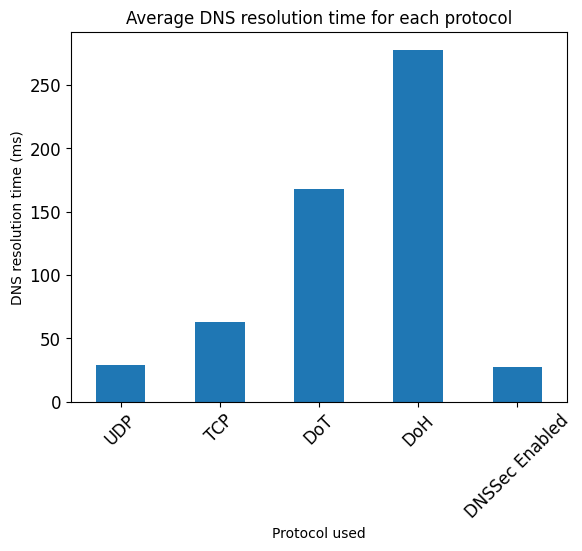
\includegraphics[width=.7\columnwidth]{images/avgLat2.1.png}
  \caption{DNS query resolution time for different DNS protocols and security implementations}
  \label{fig-5}
\end{figure}

\subsubsection*{2. Measure the performance of different Name Servers when processing the same
  set of queries. Does the performance vary with the Name Server? Does it depend
  on the type of query or on the geographic location of the Name Server?}
To accurately measure the performance of different name servers, the dnseval command was utilized to query the name servers of the local DNS servers.
In this experiment, a set of standardized queries were used to analyse which factors can affect the DNS performance.
The name servers tested were located around the world (Table \ref*{tab-7}) to provide a comprehensive evaluation of performance across different regions,
for each of them 600 queries were performed for each query type.
\rowcolors{2}{green!8}{green!18}
\begin{table}[H]
  \centering
  \begin{tabular}{|c|c|}
    \hline
    \linewidth=0cm
    Location & ip              \\
    \hline
    America  & 108.162.46.243  \\
    Japan    & 203.141.131.66  \\
    France   & 188.165.187.102 \\
    \hline
  \end{tabular}
  \caption{Location and ip address of local name servers used}
  \label{tab-7}
\end{table}

As demonstrated by the graph in Figure \ref{fig-6}, the type of DNS query used does not have a significant impact on query resolution time.
This may be attributed to the fact that the different query types for Google have a similar number of records,
resulting in similar processing and sending times for each query.
However, it is important to note that this finding may not apply universally to all DNS queries, as variations in record counts or other factors may lead to different results.
Further research could be conducted to investigate the impact of query type on DNS performance under different conditions.

\begin{figure}[H]
  \centering
  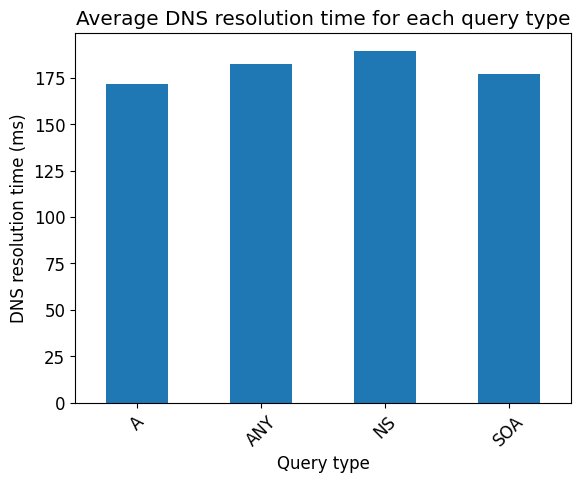
\includegraphics[width=.7\columnwidth]{images/latQueryType.png}
  \caption{DNS query resolution time for query type}
  \label{fig-6}
\end{figure}


In contrast, the location of the different nameservers has a significant impact on DNS resolution time,
with name servers located closer to Pavia having shorter resolution times than those located further away.\\
As shown in Figure \ref{fig-7}, the nameserver located in France has a lower resolution time compared to those located in America and Japan.
That is because name server in France is physically closer to Pavia than the ones in America and Japan, resulting in a lower resolution time.
So, the distance that the DNS query has to travel is shorter, and there are fewer network nodes or routers that the query has to pass through, leading to less latency or delay in the response.
\begin{figure}[H]
  \centering
  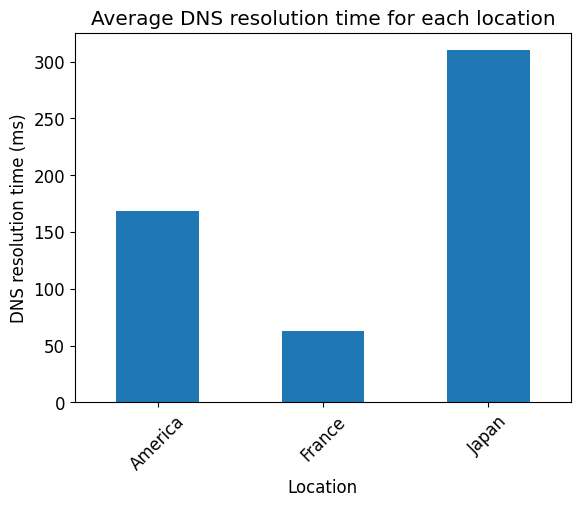
\includegraphics[width=.7\columnwidth]{images/avgLat2.2.loc.png}
  \caption{DNS query resolution time for each DNS servers}
  \label{fig-7}
\end{figure}
\subsubsection*{3. Check the path followed by your queries using different Name Servers; does the
  performance depend on the number of hops? Did you notice any
  expected/unexpected behavior?}

To perform a sufficient number of queries, a bash script was created to execute 100 dnstraceroute tests for each name server throughout the day.\\
The results, shown in Figures \ref{fig-8} and \ref{fig-9}, indicate that latency is not necessarily correlated with the number of hops,
as evidenced by openDNS having the highest latency but the lowest number of hops.
Conversely, Google has a high number of hops compared to the others but the lowest latency.
This phenomenon may be due to the fact that the number of hops does not have a significant impact on latency,
but rather latency is influenced by the physical distance between the DNS server and the client.
Other factors such as network congestion, routing policies, and hardware capabilities may also affect latency and must be taken into consideration.

\begin{figure}[H]
  \centering
  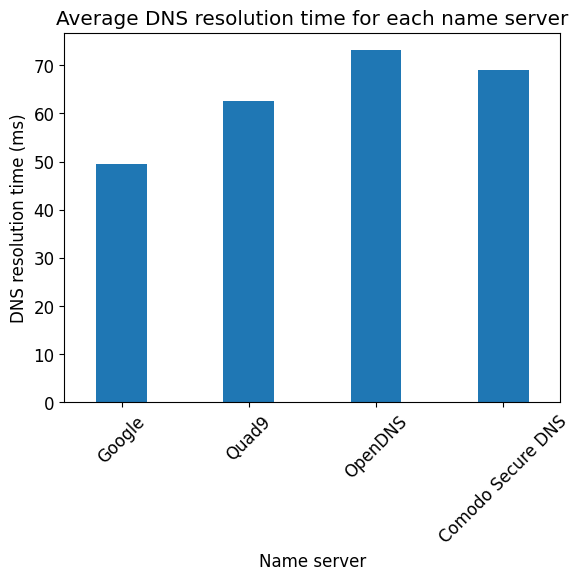
\includegraphics[width=.7\columnwidth]{images/avgLat2.3.png}
  \caption{Average latency for each local name servers}
  \label{fig-8}
\end{figure}

\begin{figure}[H]
  \centering
  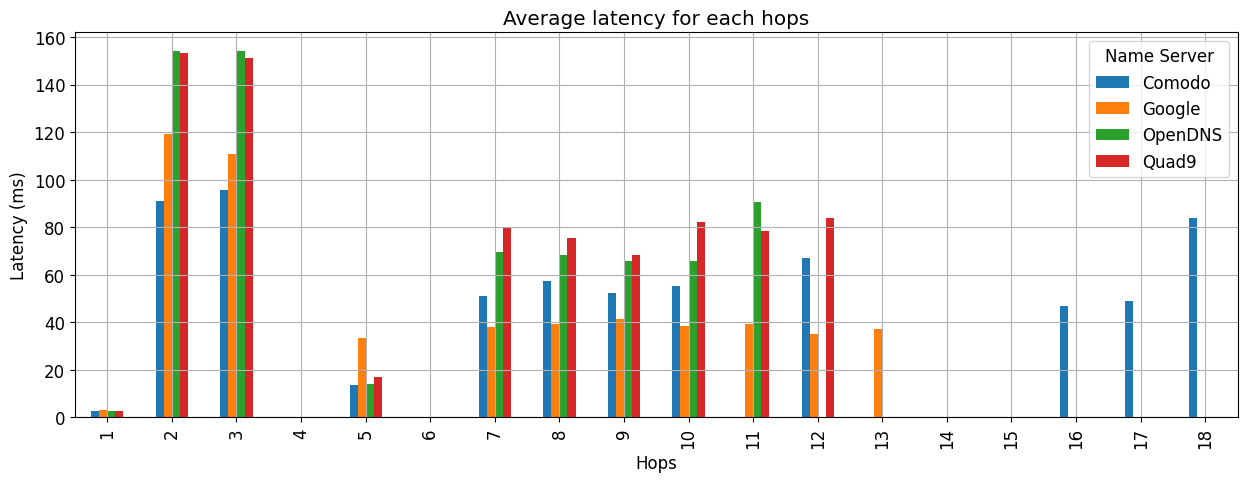
\includegraphics[width=\columnwidth]{images/avglathops2.3.png}
  \caption{Average latency for query type and for each hops of DNS servers}
  \label{fig-9}
\end{figure}
\section{Conclusions}
In conclusion, this report has provided two analyses of network performance with regards to ProtonVPN servers and DNS servers.
The first analysis explored the impact of server location on network performance by measuring latency, packet loss, and network bandwidth of various ProtonVPN servers.
The second analysis focused on DNS performance, studying the contents of DNS queries and responses, and evaluating the performance of different DNS servers and protocols.
The results of these analyses provide valuable insights into optimizing server selection to achieve optimal network performance, privacy, and security for users.
The findings suggest that selecting ProtonVPN servers that are closer to the user's location can significantly improve network performance.
Furthermore, the study demonstrates the importance of DNS performance in network performance, as DNS queries are a critical component of network communication.

\end{document}